% ============================================================
%  SPICE Exercises — Progress Presentation
%  Compiled with: pdflatex or xelatex
% ============================================================
\documentclass[aspectratio=169, 10pt]{beamer}

% ── Theme & Colors ──────────────────────────────────────────
\usetheme{metropolis}
\usepackage{appendixnumberbeamer}

% Custom palette — deep navy + electric accent
\definecolor{PrimaryDark}{HTML}{0D1B2A}
\definecolor{PrimaryMid}{HTML}{1B2838}
\definecolor{AccentBlue}{HTML}{00B4D8}
\definecolor{AccentTeal}{HTML}{00F5D4}
\definecolor{TextLight}{HTML}{E0E1DD}
\definecolor{SoftGray}{HTML}{778DA9}
\definecolor{CodeBG}{HTML}{1E293B}
\definecolor{HighlightBox}{HTML}{0A2342}

\setbeamercolor{normal text}{fg=TextLight, bg=PrimaryDark}
\setbeamercolor{alerted text}{fg=AccentTeal}
\setbeamercolor{example text}{fg=AccentBlue}
\setbeamercolor{title}{fg=white, bg=PrimaryDark}
\setbeamercolor{title separator}{fg=AccentBlue}
\setbeamercolor{frame title}{fg=white, bg=PrimaryMid}
\setbeamercolor{progress bar}{fg=AccentBlue, bg=PrimaryMid}
\setbeamercolor{block title}{fg=white, bg=AccentBlue!80!black}
\setbeamercolor{block body}{fg=TextLight, bg=HighlightBox}
\setbeamercolor{block title alerted}{fg=white, bg=red!70!black}
\setbeamercolor{block body alerted}{fg=TextLight, bg=HighlightBox}
\setbeamercolor{block title example}{fg=white, bg=AccentTeal!70!black}
\setbeamercolor{block body example}{fg=TextLight, bg=HighlightBox}
\setbeamercolor{footnote}{fg=SoftGray}
\setbeamercolor{footline}{fg=SoftGray}
\setbeamercolor{item}{fg=AccentBlue}

\setbeamerfont{title}{size=\Large, series=\bfseries}
\setbeamerfont{subtitle}{size=\normalsize}
\setbeamerfont{frame title}{size=\large, series=\bfseries}

% ── Packages ────────────────────────────────────────────────
\usepackage[utf8]{inputenc}
\usepackage{graphicx}
\usepackage{amsmath, amssymb}
\usepackage{booktabs}
\usepackage{listings}
\usepackage{tikz}
\usepackage{multicol}
\usepackage{xcolor}
\usepackage{hyperref}
\usetikzlibrary{shapes.geometric, arrows.meta, positioning, calc}

% ── Code listings style ────────────────────────────────────
\lstdefinestyle{spectrestyle}{
    backgroundcolor=\color{CodeBG},
    basicstyle=\ttfamily\scriptsize\color{TextLight},
    commentstyle=\color{AccentTeal!70},
    keywordstyle=\color{AccentBlue}\bfseries,
    stringstyle=\color{AccentTeal},
    numbers=left,
    numberstyle=\tiny\color{SoftGray},
    numbersep=6pt,
    breaklines=true,
    frame=none,
    xleftmargin=10pt,
    xrightmargin=5pt,
    aboveskip=8pt,
    belowskip=5pt,
    tabsize=2
}
\lstset{style=spectrestyle}

% ── Meta ────────────────────────────────────────────────────
\title{SPICE Exercises}
\subtitle{Progress Report — Cadence Spectre Simulations}
\author{PhD Preparation \textemdash\ SPICE Proficiency}
\date{\today}
\institute{Based on exercises by Prof.\ Sunil Khatri, Texas A\&M University}

% ============================================================
\begin{document}

% ── Title ───────────────────────────────────────────────────
{
\setbeamertemplate{footline}{}
\begin{frame}[standout]
    \titlepage
\end{frame}
}

% ── Outline ─────────────────────────────────────────────────
\begin{frame}{Outline}
    \setbeamertemplate{section in toc}[sections numbered]
    \tableofcontents[hideallsubsections]
\end{frame}

% ============================================================
% SECTION 1: Control Statements
% ============================================================
\section{Control Statements}

\begin{frame}{Control Statements — Overview}
    Spectre provides several control statements for dynamic simulation management:
    \vspace{0.5em}
    \begin{columns}[T]
        \begin{column}{0.32\textwidth}
            \begin{block}{\texttt{alter}}
                Modify parameters between analysis runs without restarting the simulator.
            \end{block}
        \end{column}
        \begin{column}{0.32\textwidth}
            \begin{block}{\texttt{info}}
                Extract specific component parameters and route output to the logfile.
            \end{block}
        \end{column}
        \begin{column}{0.32\textwidth}
            \begin{block}{\texttt{simstat}}
                Profile memory usage and CPU time for performance analysis.
            \end{block}
        \end{column}
    \end{columns}
\end{frame}

\begin{frame}[fragile]{Dynamic Parameter Modification — \texttt{alter}}
    \begin{columns}[T]
        \begin{column}{0.45\textwidth}
            The \texttt{alter} statement changes parameters between distinct analysis runs:
            \vspace{0.5em}
            \begin{lstlisting}[language=C]
// DC analysis at nominal temp
dc1 dc oppoint=logfile
     homotopy=gmin

// Change temp, run transient
Change1 alter param=temp
        value=100
tran1 tran stop=1u
            \end{lstlisting}
        \end{column}
        \begin{column}{0.52\textwidth}
            \centering
            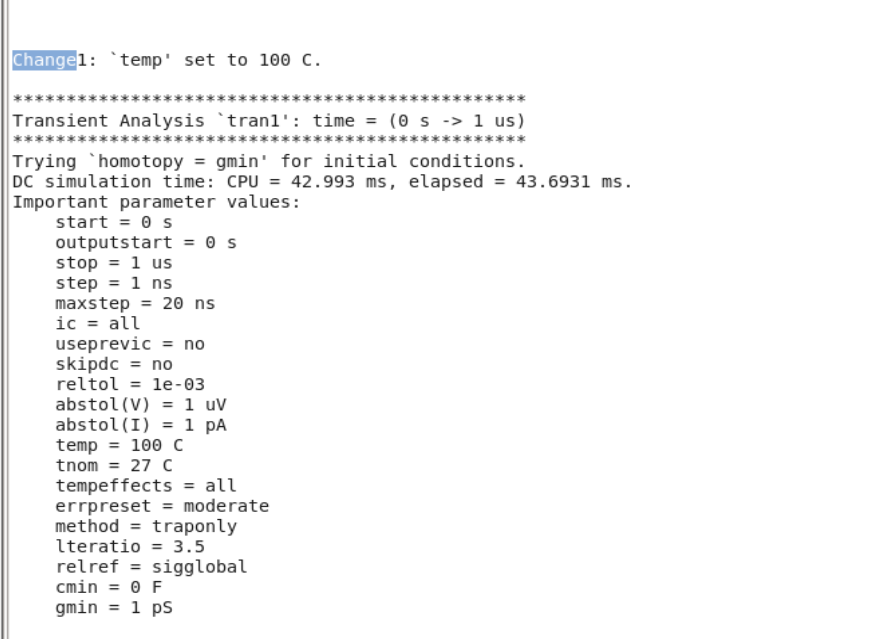
\includegraphics[width=\textwidth]{SPECTRE/Control_statements/change_in_temperature_parameter_via_alter_statement.png}
            \vspace{0.3em}
            {\scriptsize Temperature modification via \texttt{alter}.}
        \end{column}
    \end{columns}
\end{frame}

\begin{frame}{Data Extraction \& Performance Profiling}
    \begin{columns}[T]
        \begin{column}{0.48\textwidth}
            \begin{block}{\texttt{info} — Output Extraction}
                Extracts specific component parameters and routes them directly to the logfile.
            \end{block}
            \vspace{0.3em}
            \centering
            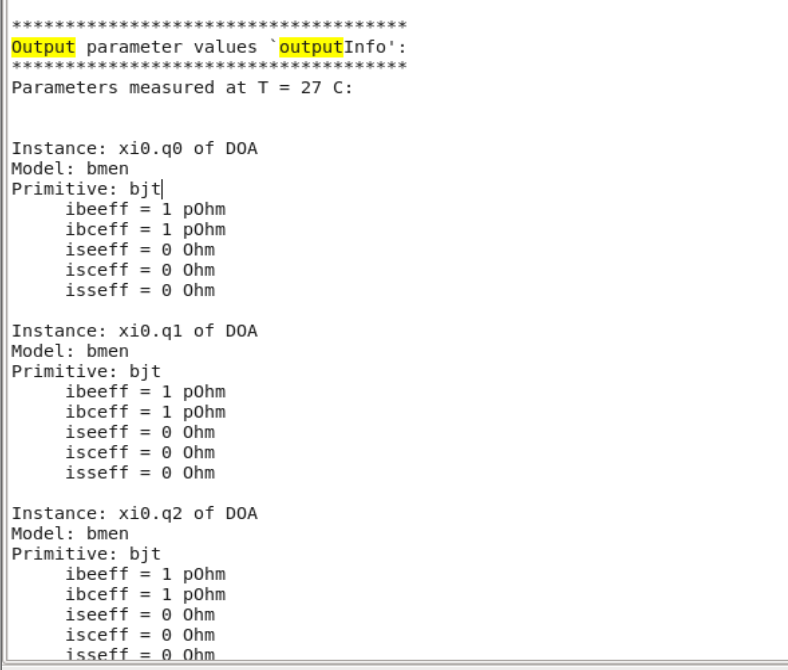
\includegraphics[width=0.95\textwidth]{SPECTRE/Control_statements/use_of_info_control_statement.png}
        \end{column}
        \begin{column}{0.48\textwidth}
            \begin{block}{\texttt{simstat} — Performance Profiling}
                Setting \texttt{simstat=detailed} provides in-depth memory and CPU breakdowns.
            \end{block}
            \vspace{0.3em}
            \centering
            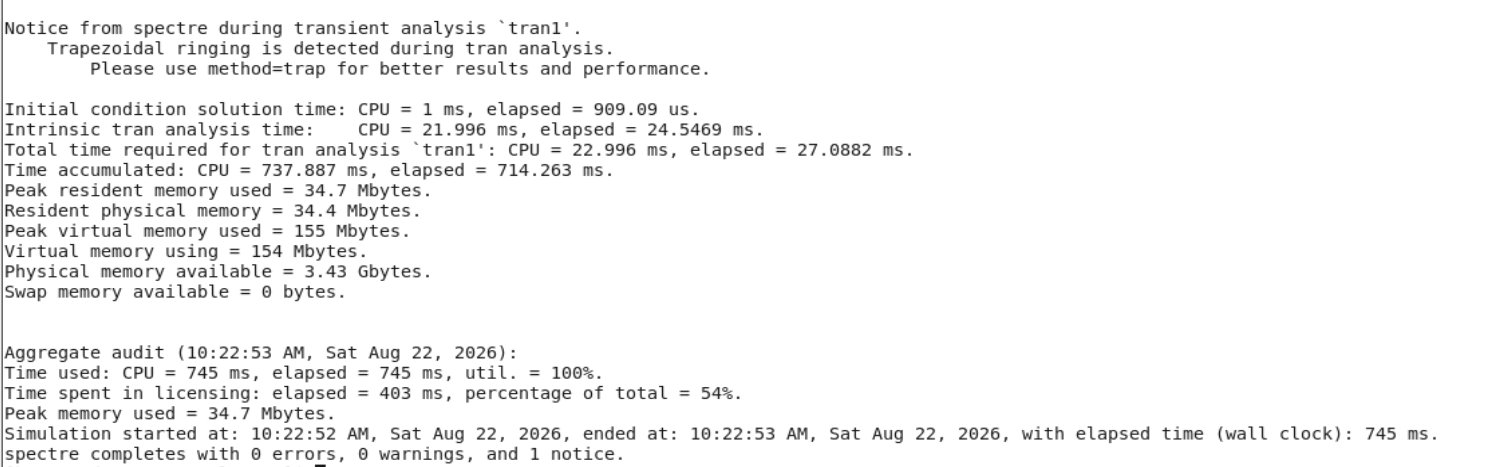
\includegraphics[width=0.95\textwidth]{SPECTRE/Control_statements/simstat_detailed_output.png}
        \end{column}
    \end{columns}
\end{frame}

% ============================================================
% SECTION 2: Temperature vs Trise
% ============================================================
\section{Temperature vs Trise}

\begin{frame}{Temperature Handling in Device Models}
    \begin{columns}[T]
        \begin{column}{0.55\textwidth}
            Two key parameters control device temperature:
            \vspace{0.8em}
            \begin{exampleblock}{\texttt{temp} — Exclusive}
                Overrides the ambient temperature setting entirely.
            \end{exampleblock}
            \vspace{0.5em}
            \begin{alertblock}{\texttt{trise} — Accumulative}
                Adds on top of the current ambient temperature.
            \end{alertblock}
            \vspace{0.8em}
            \alert{Key insight:} These behave fundamentally differently when combined with global temperature settings.
        \end{column}
        \begin{column}{0.42\textwidth}
            \centering
            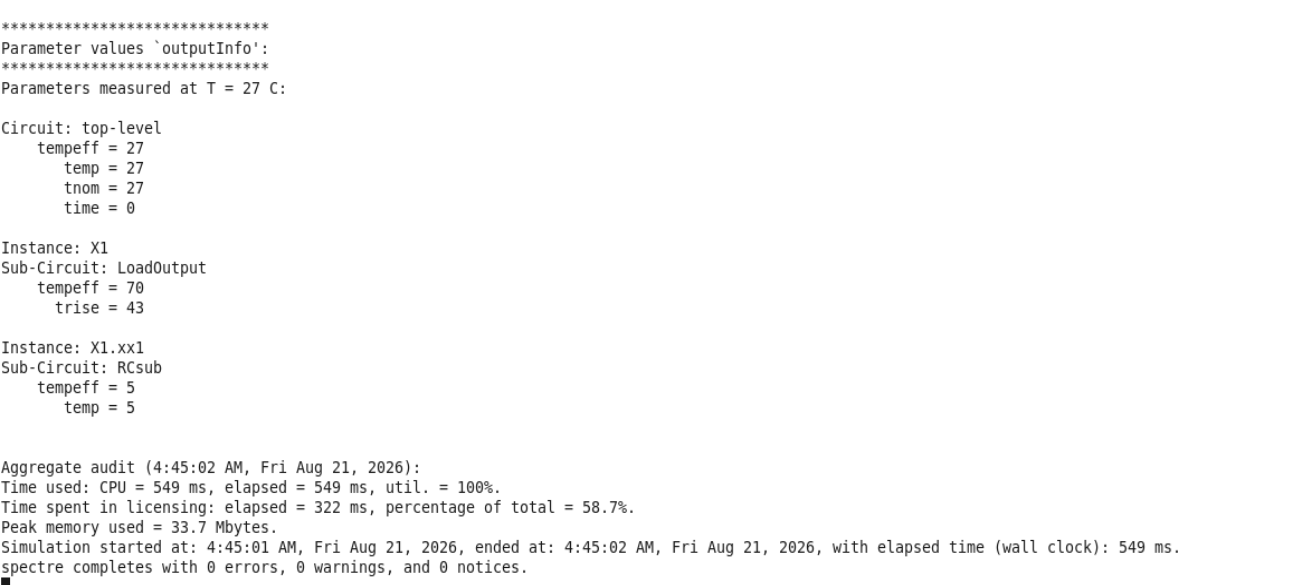
\includegraphics[width=\textwidth]{SPECTRE/temp_vs_trise/demo_showing_accumulative_nature_of_trise_and_exclusive_nature_of_temp_same_time.png}
            \vspace{0.3em}
            {\scriptsize Combined effect: \texttt{trise} accumulates while \texttt{temp} overrides.}
        \end{column}
    \end{columns}
\end{frame}

\begin{frame}{\texttt{temp} vs \texttt{trise} — Individual Demonstrations}
    \begin{columns}[c]
        \begin{column}{0.48\textwidth}
            \centering
            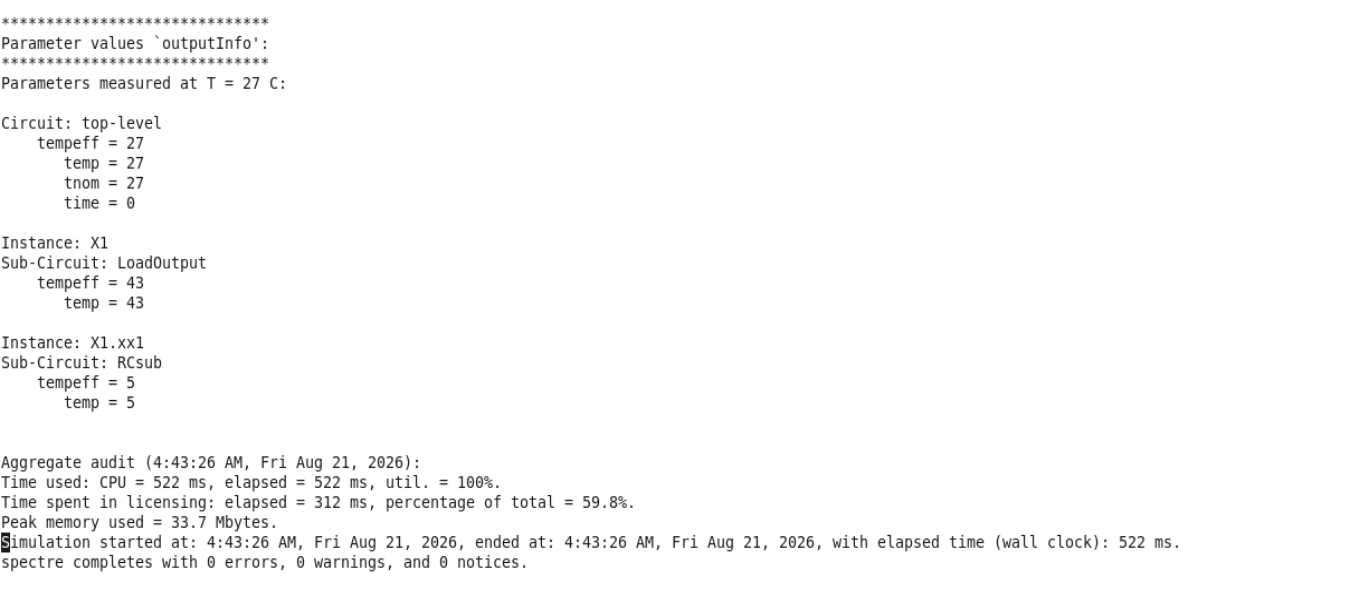
\includegraphics[width=\textwidth]{SPECTRE/temp_vs_trise/temp_command_exclusive_temperature.png}
            \vspace{0.3em}
            {\scriptsize Exclusive nature of \texttt{temp}.}
        \end{column}
        \begin{column}{0.48\textwidth}
            \centering
            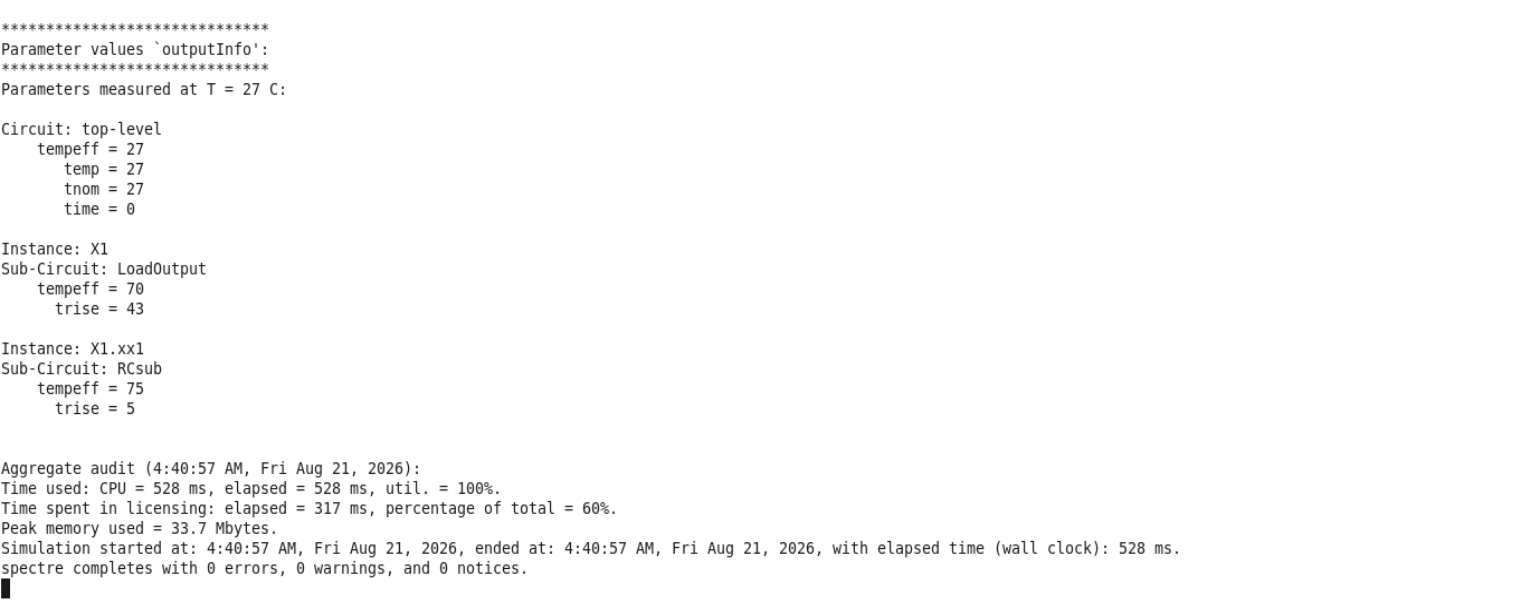
\includegraphics[width=\textwidth]{SPECTRE/temp_vs_trise/trise_accumulative_effect_demo.png}
            \vspace{0.3em}
            {\scriptsize Accumulative nature of \texttt{trise}.}
        \end{column}
    \end{columns}
\end{frame}

% ============================================================
% SECTION 3: Exercise 1
% ============================================================
\section{Exercise 1: CMOS Inverter Chain}

\begin{frame}{Exercise 1 — Setup}
    \begin{block}{Circuit Configuration}
        7-stage CMOS inverter chain \textemdash\ 22-nm PTM HP model.
    \end{block}
    \vspace{0.5em}
    \begin{columns}[T]
        \begin{column}{0.45\textwidth}
            \textbf{Design Parameters:}
            \begin{table}
                \centering
                \begin{tabular}{@{}ll@{}}
                    \toprule
                    Parameter & Value \\
                    \midrule
                    $L$ & 22 nm \\
                    $W_n$ & 44 nm \\
                    $W_p$ & $k \times W_n$ \\
                    $V_{DD}$ & 1 V \\
                    \bottomrule
                \end{tabular}
            \end{table}
        \end{column}
        \begin{column}{0.52\textwidth}
            \textbf{Measurement Methodology:}
            \begin{itemize}
                \item Propagation delays ($t_{PHL}$, $t_{PLH}$) at 50\% $V_{DD}$
                \item Rise time ($t_{rise}$) and fall time ($t_{fall}$) at 10\%--90\% thresholds
                \item Parametric sweeps of $k$ and input transition time $X$
            \end{itemize}
        \end{column}
    \end{columns}
\end{frame}

% ── Smoke Test ──────────────────────────────────────────────
\begin{frame}{Initial Smoke Test — $k = 2$}
    \begin{columns}[c]
        \begin{column}{0.48\textwidth}
            \centering
            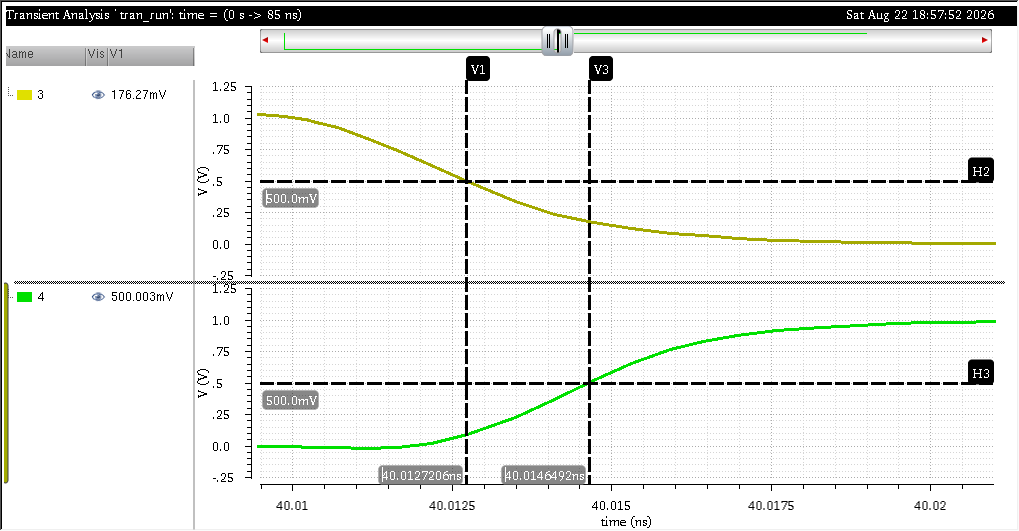
\includegraphics[width=\textwidth]{SPECTRE/Exercise1/TPHL_INVERTER_CHAIN_K_IS_2.png}
            \vspace{0.2em}
            {\scriptsize $t_{PHL} \approx 1.9286$ ps}
        \end{column}
        \begin{column}{0.48\textwidth}
            \centering
            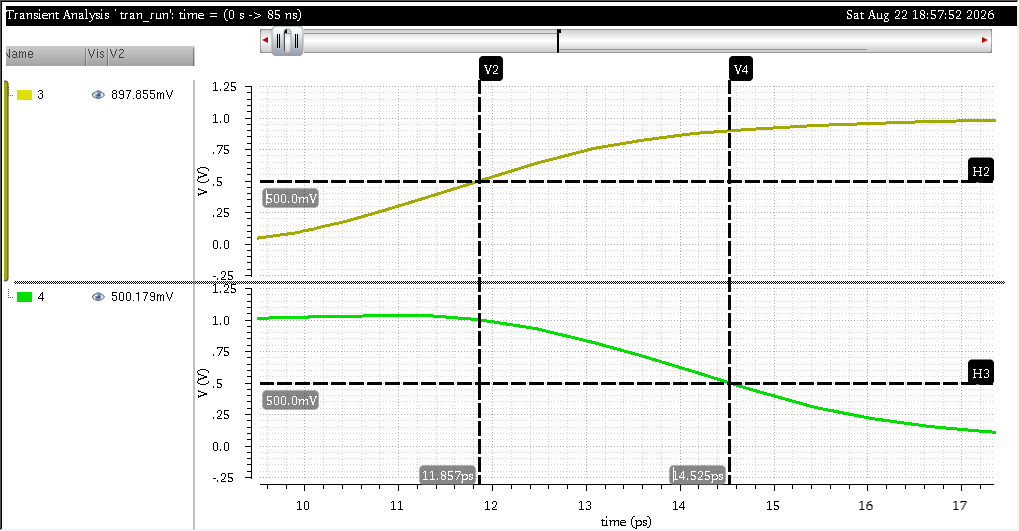
\includegraphics[width=\textwidth]{SPECTRE/Exercise1/TPLH_INVERTER_CHAIN_K_IS_2.png}
            \vspace{0.2em}
            {\scriptsize $t_{PLH} \approx 2.668$ ps}
        \end{column}
    \end{columns}
    \vspace{0.8em}
    \centering
    \begin{block}{Observation}
        $t_{PLH} > t_{PHL}$ \quad$\Longrightarrow$\quad PMOS is weaker than NMOS at $k = 2$.
    \end{block}
\end{frame}

% ── Part A: Propagation Delays ──────────────────────────────
\begin{frame}{Part A — $t_{PHL}$ vs $t_{PLH}$ as a Function of $k$}
    \begin{columns}[c]
        \begin{column}{0.48\textwidth}
            \centering
            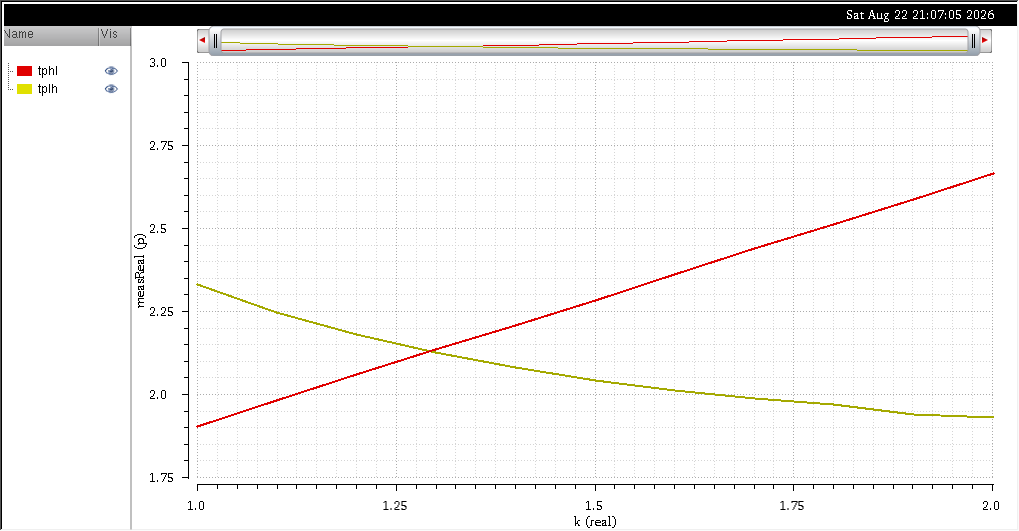
\includegraphics[width=\textwidth]{SPECTRE/Exercise1/tplh_vs_tphl_as_a_function_of_k.png}
            \vspace{0.2em}
            {\scriptsize Spectre parametric sweep result.}
        \end{column}
        \begin{column}{0.48\textwidth}
            \centering
            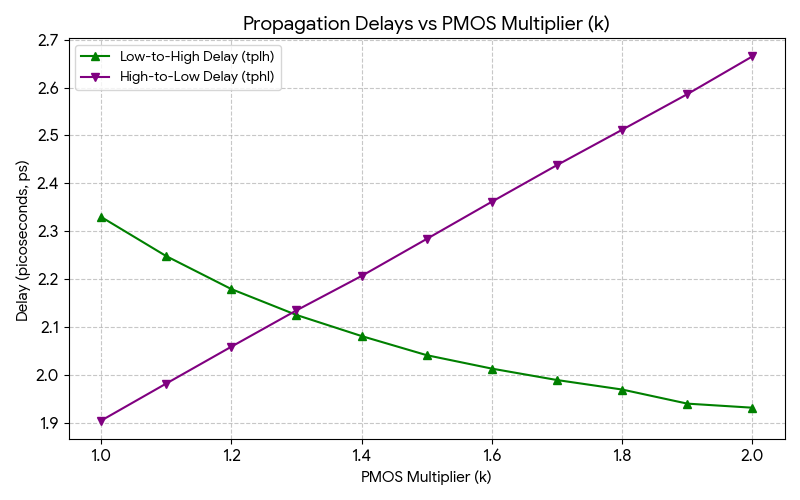
\includegraphics[width=\textwidth]{SPECTRE/Exercise1/tplh_vs_tphl_python_generated.png}
            \vspace{0.2em}
            {\scriptsize Python-generated verification plot.}
        \end{column}
    \end{columns}
    \vspace{0.5em}
    \centering
    \begin{block}{Result}
        Curves intersect at \alert{$k \approx 1.293$}, where $t_{PHL} \approx t_{PLH} \approx 2.13$ ps.
    \end{block}
\end{frame}

\begin{frame}{Part A — Calculator Verification}
    \begin{columns}[c]
        \begin{column}{0.55\textwidth}
            The Spectre calculator utility independently confirms the intersection point:
            \vspace{0.8em}
            \begin{exampleblock}{Verified Result}
                \centering
                \large
                $\boxed{k \approx 1.293}$
                \vspace{0.3em}

                $t_{PHL} \approx t_{PLH} \approx 2.13\text{ ps}$
            \end{exampleblock}
        \end{column}
        \begin{column}{0.42\textwidth}
            \centering
            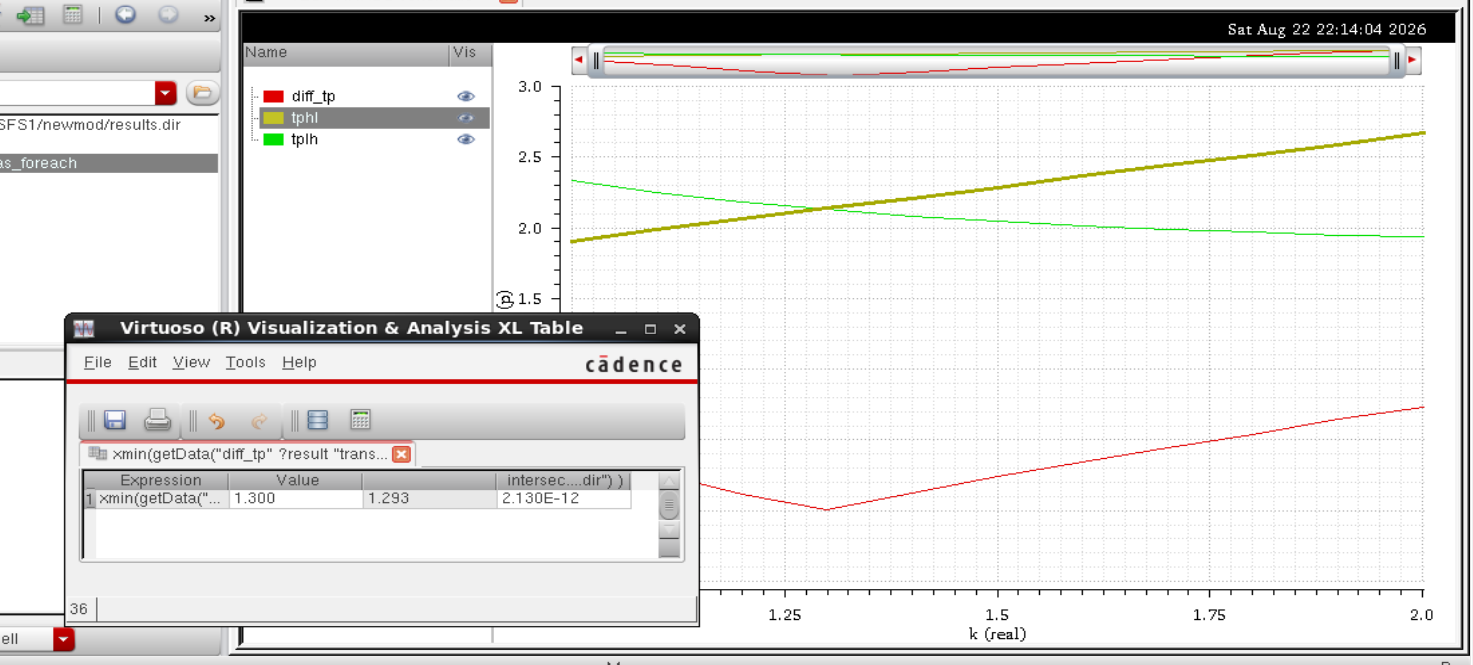
\includegraphics[width=\textwidth]{SPECTRE/Exercise1/k_value_for_tplh_equal_tphl_from_calc_utility.png}
            \vspace{0.3em}
            {\scriptsize Calculator utility output.}
        \end{column}
    \end{columns}
\end{frame}

% ── Part A: Rise / Fall Times ───────────────────────────────
\begin{frame}{Part A — $t_{rise}$ vs $t_{fall}$ as a Function of $k$}
    \begin{columns}[c]
        \begin{column}{0.48\textwidth}
            \centering
            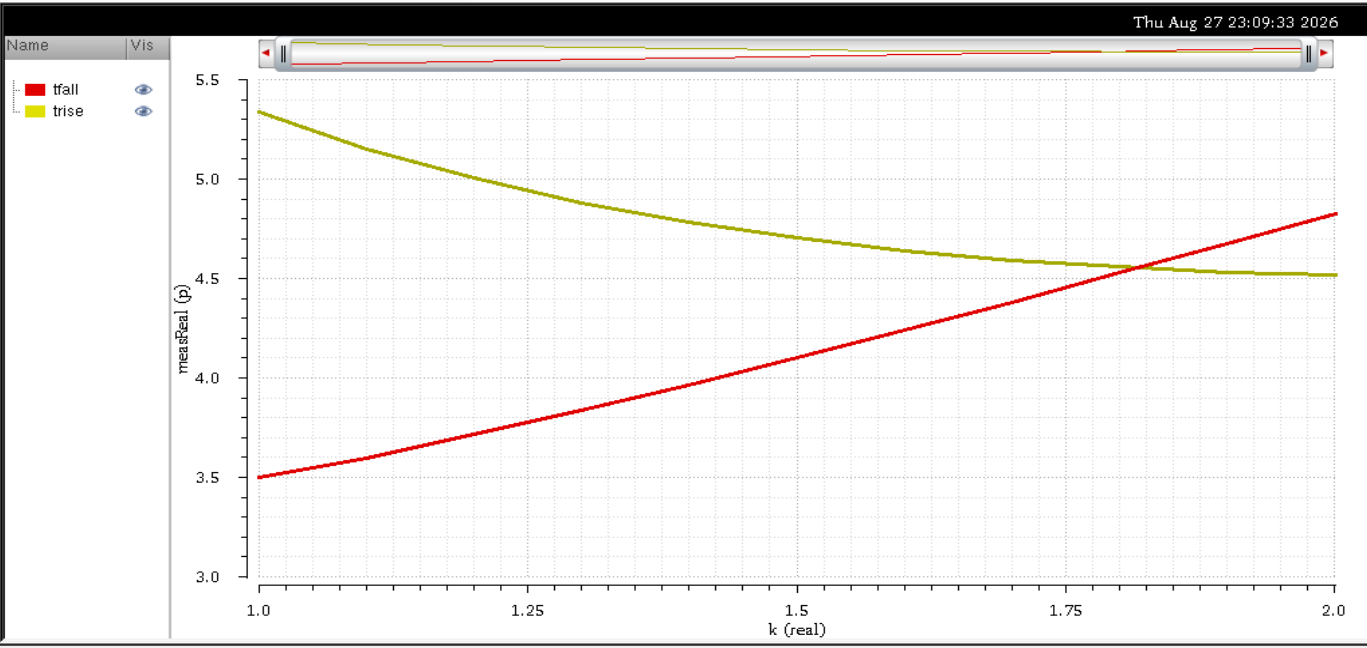
\includegraphics[width=\textwidth]{SPECTRE/Exercise1/trise_vs_tfall_values_as_k_is_swept_at_x_of10p.png}
            \vspace{0.2em}
            {\scriptsize Spectre parametric sweep result.}
        \end{column}
        \begin{column}{0.48\textwidth}
            \centering
            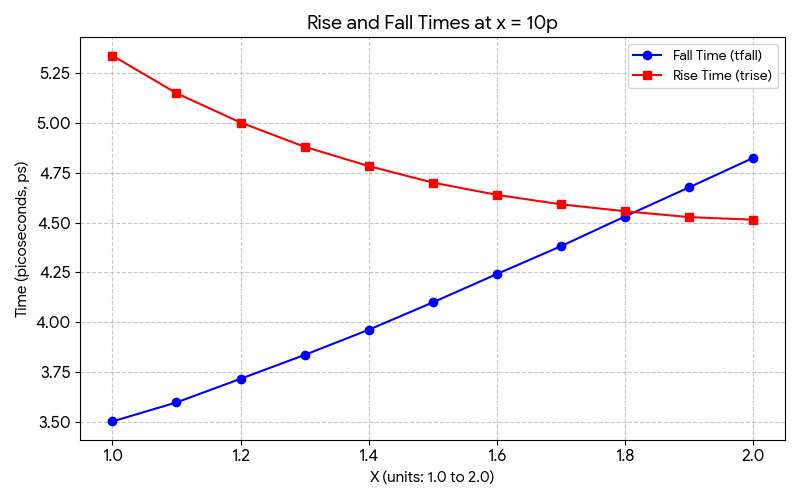
\includegraphics[width=\textwidth]{SPECTRE/Exercise1/trise_vs_tfall_python_generated.png}
            \vspace{0.2em}
            {\scriptsize Python-generated verification plot.}
        \end{column}
    \end{columns}
    \vspace{0.5em}
    \centering
    \begin{block}{Result}
        Rise and fall times are equal at \alert{$k \approx 1.82$}, where $t_{rise} \approx t_{fall} \approx 4.55$ ps.
    \end{block}
\end{frame}

% ── Part A: Summary ─────────────────────────────────────────
\begin{frame}{Part A — Summary of Findings}
    \centering
    \begin{table}
        \centering
        \begin{tabular}{@{}lcc@{}}
            \toprule
            \textbf{Condition} & \textbf{$k$ value} & \textbf{Symmetric delay} \\
            \midrule
            $t_{PHL} = t_{PLH}$ & 1.293 & 2.13 ps \\
            $t_{rise} = t_{fall}$ & 1.82 & 4.55 ps \\
            \bottomrule
        \end{tabular}
    \end{table}
    \vspace{1em}
    \begin{alertblock}{Key Observation}
        The $k$ values for symmetric propagation delay and symmetric rise/fall times are \textbf{different}. Propagation delay symmetry occurs at a lower $k$ than rise/fall time symmetry.
    \end{alertblock}
\end{frame}

% ── Part B ──────────────────────────────────────────────────
\begin{frame}{Part B — Sweep of $X$ for Symmetric $t_{rise}$ / $t_{fall}$}
    \begin{columns}[c]
        \begin{column}{0.48\textwidth}
            \centering
            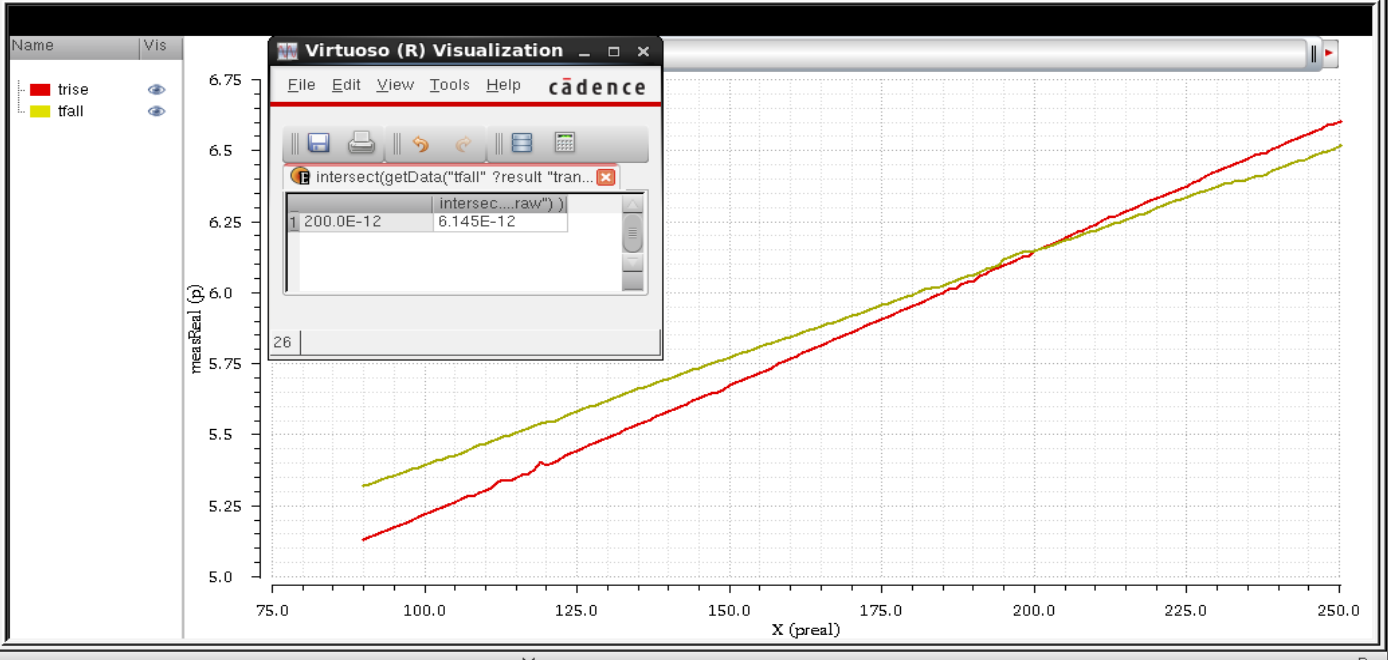
\includegraphics[width=\textwidth]{SPECTRE/Exercise1/viva_trise_tfall_as_X_is_varied_with_their_intersection_graphically_and_calculator_utility.png}
            \vspace{0.2em}
            {\scriptsize Spectre result with calculator utility.}
        \end{column}
        \begin{column}{0.48\textwidth}
            \centering
            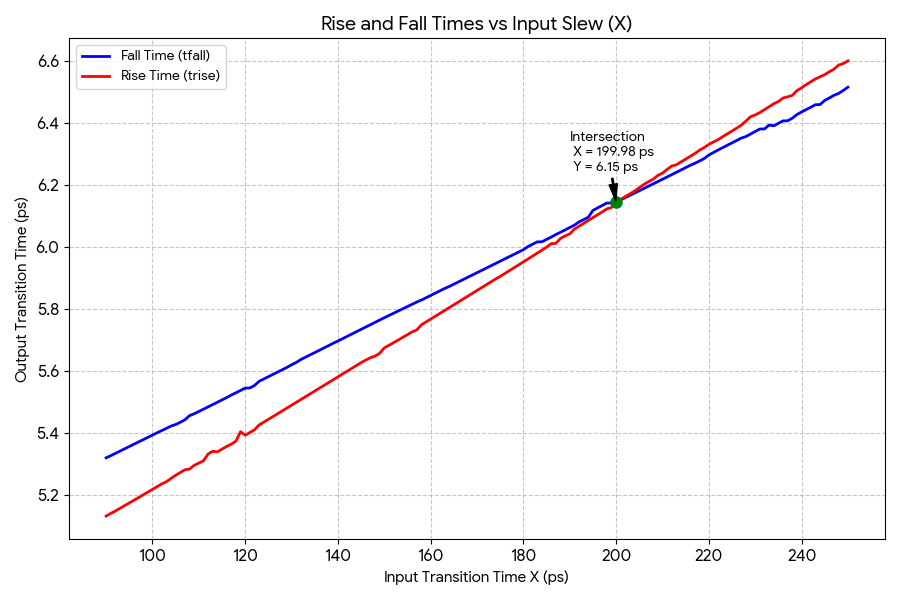
\includegraphics[width=\textwidth]{SPECTRE/Exercise1/trise_and_tfall_as_x_is_varied_python_generated.png}
            \vspace{0.2em}
            {\scriptsize Python-generated verification plot.}
        \end{column}
    \end{columns}
    \vspace{0.5em}
    \centering
    \begin{block}{Result}
        Symmetric input transition time: \alert{$X \approx 200$ ps}, where $t_{rise} \approx t_{fall} \approx 6.145$ ps.
    \end{block}
\end{frame}

% ── Part C: Propagation Delays ──────────────────────────────
\begin{frame}{Part C — $t_{PHL}$ vs $t_{PLH}$ at Symmetric $X = 200$ ps}
    \begin{columns}[c]
        \begin{column}{0.48\textwidth}
            \centering
            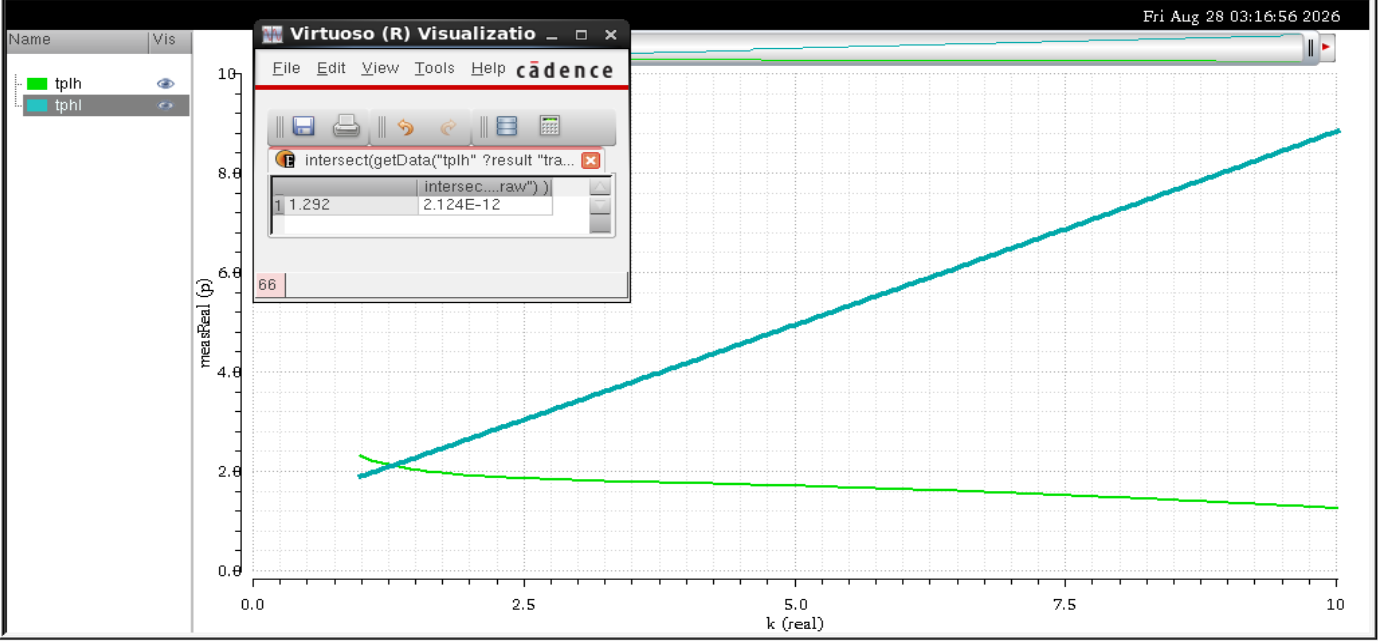
\includegraphics[width=\textwidth]{SPECTRE/Exercise1/tplh_vs_tphl_as_k_swept_for_x_at_200.png}
            \vspace{0.2em}
            {\scriptsize Spectre parametric sweep result.}
        \end{column}
        \begin{column}{0.48\textwidth}
            \centering
            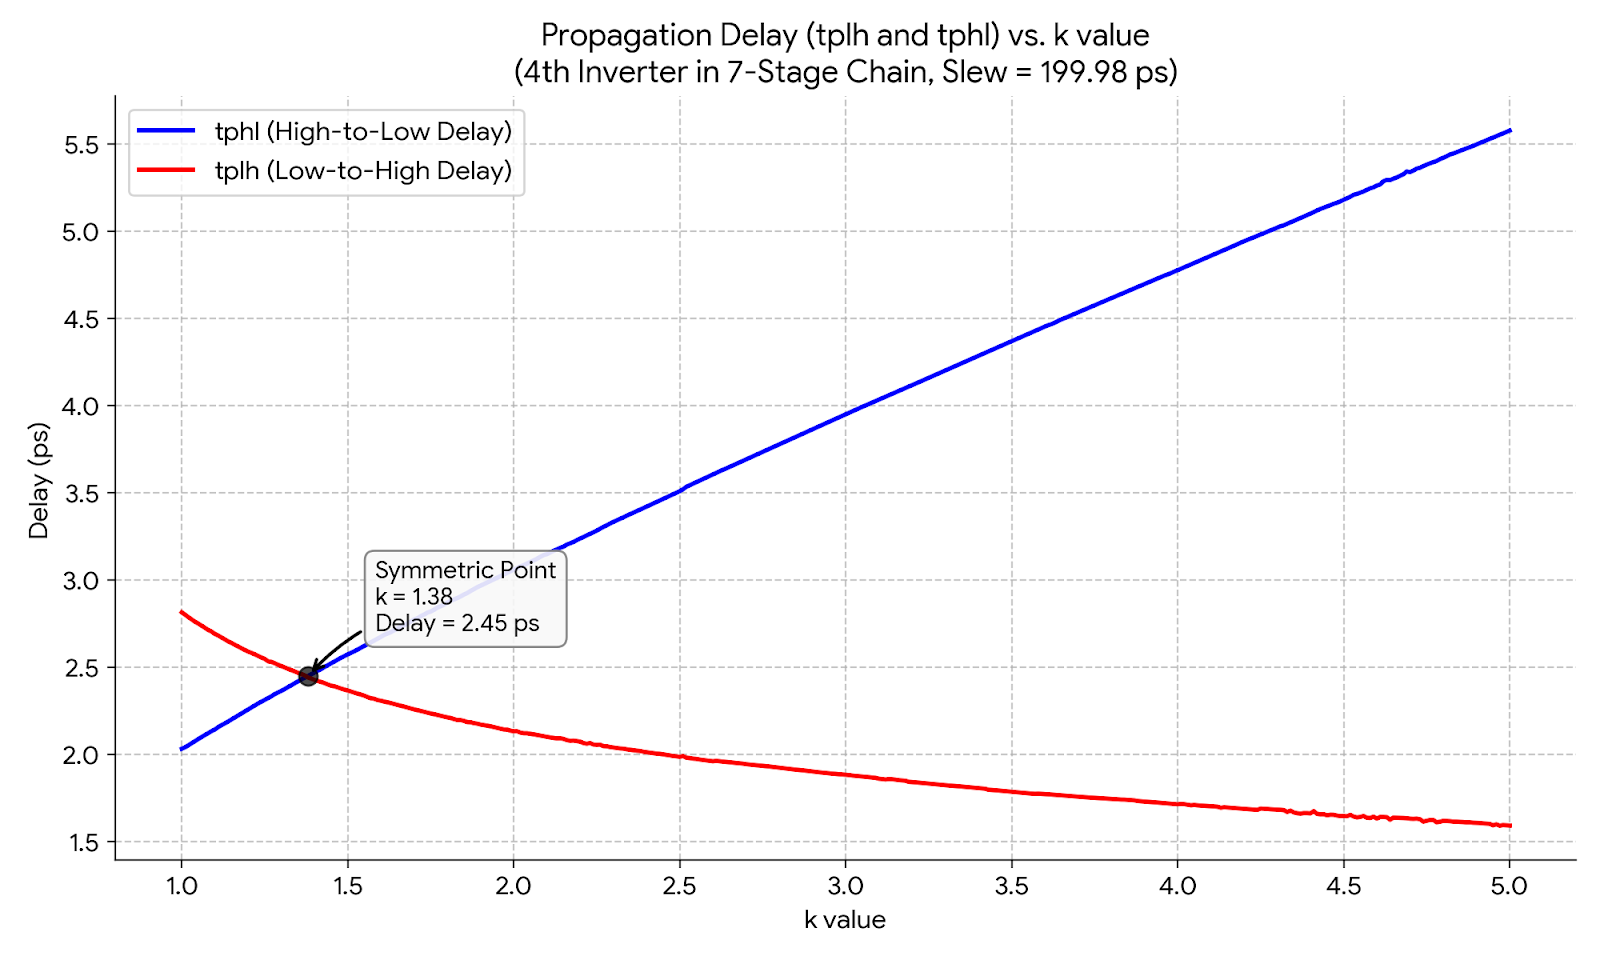
\includegraphics[width=\textwidth]{SPECTRE/Exercise1/partc_tphl_vs_tplh_as_k_is_varied_python_at_symmetric_X.png}
            \vspace{0.2em}
            {\scriptsize Python-generated verification plot.}
        \end{column}
    \end{columns}
    \vspace{0.5em}
    \centering
    \begin{block}{Result}
        \alert{$k \approx 1.38$}, with $t_{PHL} \approx t_{PLH} \approx 2.45$ ps.
        {\footnotesize (Differs from Part A's $k \approx 1.293$ due to the changed input transition time.)}
    \end{block}
\end{frame}

% ── Part C: Rise / Fall Times ───────────────────────────────
\begin{frame}{Part C — $t_{rise}$ vs $t_{fall}$ at Symmetric $X = 200$ ps}
    \begin{columns}[c]
        \begin{column}{0.48\textwidth}
            \centering
            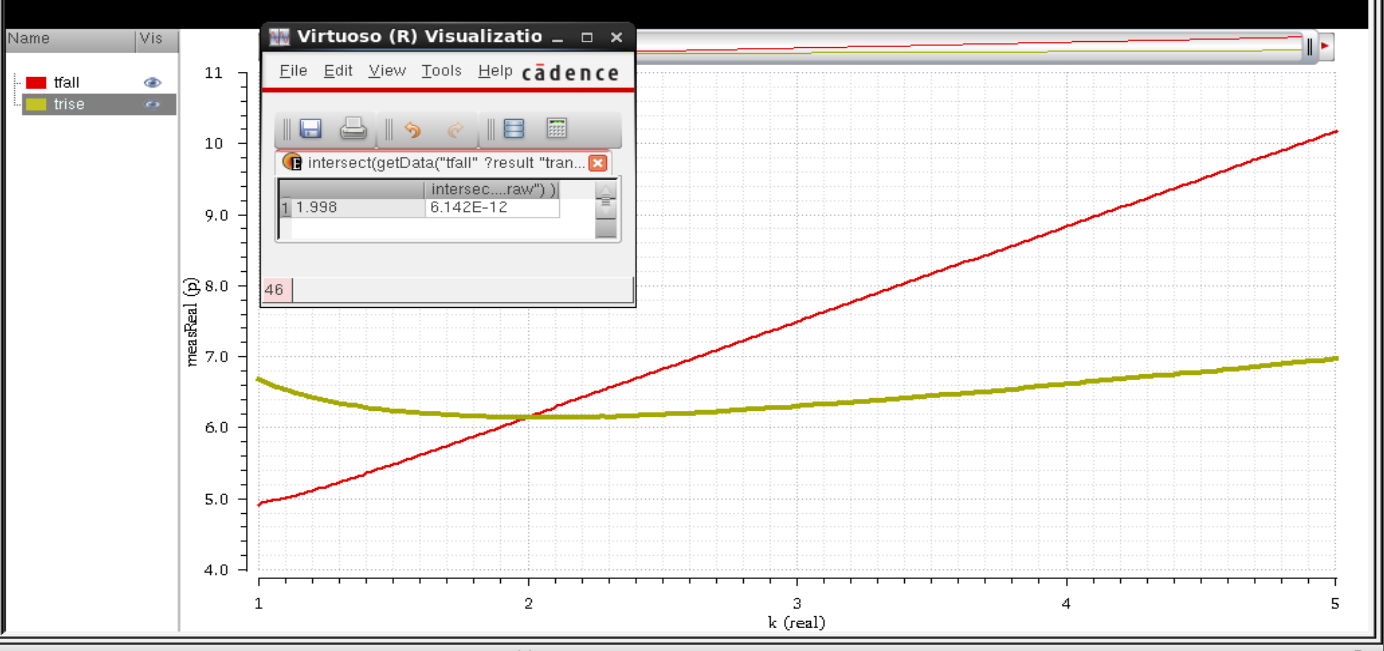
\includegraphics[width=\textwidth]{SPECTRE/Exercise1/trise_vs_tfall_as_k_swept_for_x_at_200.png}
            \vspace{0.2em}
            {\scriptsize Spectre parametric sweep result.}
        \end{column}
        \begin{column}{0.48\textwidth}
            \centering
            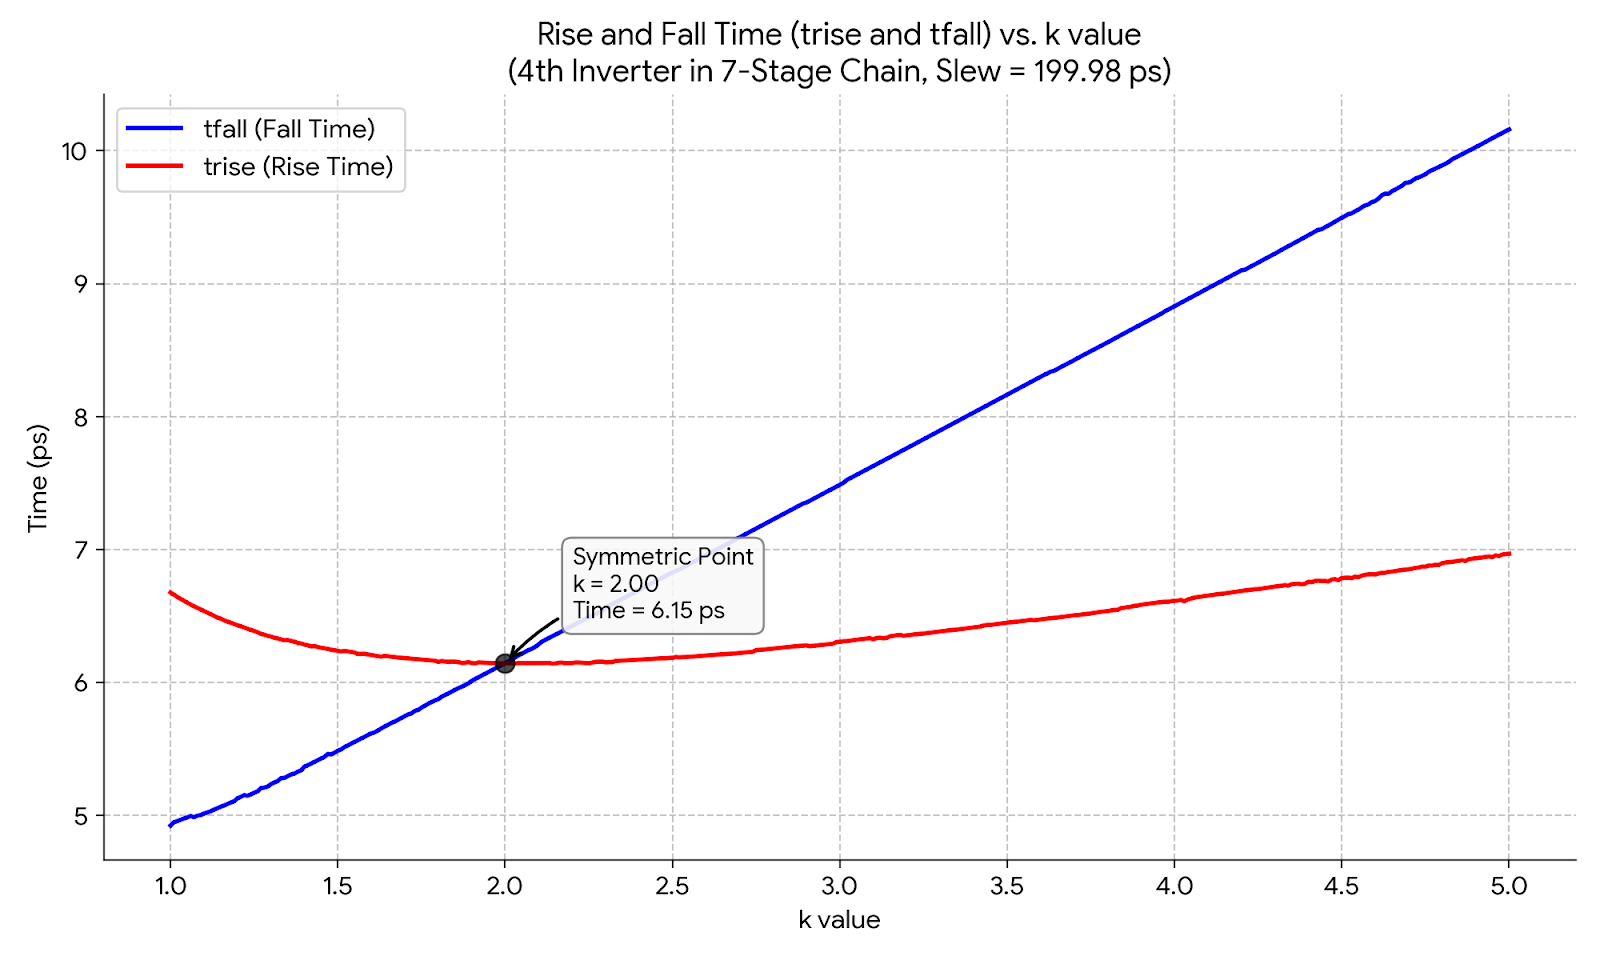
\includegraphics[width=\textwidth]{SPECTRE/Exercise1/python_partc_tr_vs_tf_t_X_symmetric_value_vs_k.png}
            \vspace{0.2em}
            {\scriptsize Python-generated verification plot.}
        \end{column}
    \end{columns}
    \vspace{0.5em}
    \centering
    \begin{block}{Result}
        \alert{$k \approx 2.0$}, with $t_{rise} \approx t_{fall} \approx 6.14$ ps.
    \end{block}
\end{frame}

% ── Part C: Summary ─────────────────────────────────────────
\begin{frame}{Exercise 1 — Consolidated Results}
    \centering
    \begin{table}
        \centering
        \begin{tabular}{@{}llcc@{}}
            \toprule
            \textbf{Part} & \textbf{Condition} & \textbf{$k$ / $X$} & \textbf{Symmetric value} \\
            \midrule
            A & $t_{PHL} = t_{PLH}$ & $k \approx 1.293$ & 2.13 ps \\
            A & $t_{rise} = t_{fall}$ & $k \approx 1.82$ & 4.55 ps \\
            \midrule
            B & $t_{rise} = t_{fall}$ (vary $X$) & $X \approx 200$ ps & 6.145 ps \\
            \midrule
            C & $t_{PHL} = t_{PLH}$ ($X = 200$ ps) & $k \approx 1.38$ & 2.45 ps \\
            C & $t_{rise} = t_{fall}$ ($X = 200$ ps) & $k \approx 2.0$ & 6.14 ps \\
            \bottomrule
        \end{tabular}
    \end{table}
    \vspace{0.8em}
    \begin{alertblock}{Takeaway}
        The input transition time ($X$) significantly affects the $k$ value required for symmetric timing. All results were cross-verified using both the Spectre calculator utility and Python scripts.
    \end{alertblock}
\end{frame}

% ============================================================
% Conclusion
% ============================================================
\section*{Conclusion}

\begin{frame}[standout]
    \large
    Significant progress through Prof.\ Khatri's SPICE exercises.

    \vspace{1em}
    \normalsize
    Strong foundation in Spectre control statements, parametric sweeps, and timing analysis established for future PhD research.

    \vspace{1.5em}
    {\small \textcolor{SoftGray}{More exercises to follow \dots}}
\end{frame}

\end{document}
